\documentclass[11pt]{article}

\usepackage[T1]{fontenc}
\usepackage{lmodern}
\usepackage[letterpaper,margin=0.78in]{geometry}
\usepackage{microtype}
\usepackage{amsmath,amssymb}
\usepackage{booktabs}
\usepackage{tabularx}
\usepackage{array}
\usepackage{longtable}
\usepackage{siunitx}
\usepackage{graphicx}
\usepackage{caption}
\usepackage{placeins}
\usepackage{float}
\usepackage{enumitem}
\usepackage[dvipsnames]{xcolor}
\usepackage{hyperref}
\usepackage{fancyhdr}
\usepackage{xurl}

\definecolor{reportblue}{HTML}{295F8A}
\definecolor{reportred}{HTML}{B33A3A}
\definecolor{reportgray}{HTML}{4D5963}
\hypersetup{
  colorlinks=true,
  linkcolor=reportblue,
  urlcolor=reportblue,
  citecolor=reportblue,
  pdftitle={Subject 15: Comparing CLOSEST occupation-density basins with direct trajectory support},
  pdfauthor={Generated from the gflowui Subject 15 analysis}
}

\captionsetup{
  font=small,
  labelfont=bf,
  justification=raggedright,
  singlelinecheck=false
}
\setlist{nosep,leftmargin=1.5em}
\setlength{\parindent}{0pt}
\setlength{\parskip}{0.48em}
\setlength{\tabcolsep}{4pt}
\renewcommand{\arraystretch}{1.08}
\sisetup{
  detect-all,
  group-separator={,},
  group-minimum-digits=4,
  group-digits=integer
}

\providecommand{\reportbuilddatetime}{unknown}
\InputIfFileExists{subject15_eot_comparison_report_build_info.tex}{}{}
\newcommand{\MassVisitSpearman}{0.973}
\newcommand{\SupportVisitSpearman}{0.464}
\newcommand{\MassVisitTV}{1.39\%}
\newcommand{\TopSeventeenMass}{more than 99.9999999999\%}
\newcommand{\DirectlyVisitedBasinCount}{17}
\newcommand{\MaximumBasinCount}{352}
\newcommand{\SubjectVisitCount}{70}
\newcommand{\ObservedSpanDays}{71}


\pagestyle{fancy}
\fancyhf{}
\fancyhead[L]{\small Subject 15 basin comparison}
\fancyhead[R]{\small \reportbuilddatetime}
\fancyfoot[C]{\thepage}
\setlength{\headheight}{14pt}

\newcommand{\rhofield}{\widehat{\rho}}
\newcommand{\R}{\mathbb{R}}
\newcommand{\keyfinding}[1]{%
  \begin{center}
  \fcolorbox{reportblue}{reportblue!5}{%
    \parbox{0.92\linewidth}{\textbf{Key finding.} #1}}
  \end{center}
}

\title{\vspace{-1.2em}\textbf{Subject 15: Comparing CLOSEST
occupation-density basins with direct trajectory support}\\[0.4em]
\large Definitions, reconstructed evidence, and implications for
elementary occupation types}
\author{\parbox{0.94\linewidth}{\centering\small
Source file:\\[-0.1em]\scriptsize
\path{~/current_projects/gflowui/dev/subject15_eot_comparison_2026-08-06/latex_report/subject15_eot_comparison_report.tex}}}
\date{\small Build \reportbuilddatetime}

\begin{document}
\maketitle
\thispagestyle{fancy}

\begin{abstract}
This report examines whether maximum basins reconstructed by discrete
\textsc{closest} ascent should be identified directly with elementary
occupation types (EOTs).  It uses the selected Subject 15 occupation-density
field, its \num{6529}-vertex graph, the \MaximumBasinCount{} reconstructed
maximum basins, and all \SubjectVisitCount{} observed subject visits.  The
analysis separates three notions that can otherwise be conflated: the number
of graph vertices assigned to a basin, the occupation-density probability mass
assigned to it, and the number of observed subject trajectory vertices that
fall in it.  All observed visits fall in M1--M17, and those 17 basins carry
numerically all density mass.  Density mass and direct visit frequency agree
closely, whereas graph support is only moderately associated with direct visit
frequency.  The singleton M17 basin is a valid discrete local maximum: its
zero-step ascent path terminates at itself even though each neighboring vertex
chooses a closer uphill route to M1.  These results support treating
\textsc{closest} basins as candidate geometric catchments and applying an
explicit subject-support criterion before interpreting them as major EOTs.
\end{abstract}

\keyfinding{For Subject 15, the apparent proliferation to 352 local-maximum
basins is almost entirely a numerical tail phenomenon: M1--M17 contain all 70
observed visits and \TopSeventeenMass{} of the reconstructed density mass.
Direct trajectory support, not graph support alone, is therefore the most
transparent additional criterion for deciding which candidate basins are
scientifically material.}

\section{Question and data}

The scientific question is not whether the discrete \textsc{closest}
construction is internally valid.  It is whether every basin produced by that
construction should be interpreted as a major elementary occupation type.
Smooth-field intuition suggests that a local maximum has a nontrivial
attraction neighborhood.  On a finite, nonsmooth graph, however, a strict local
maximum can have a basin containing only itself: every adjacent vertex may
have another higher neighbor connected by a shorter edge.

The analysis uses the selected field
\texttt{HMP\_S15\_K03\_ETA\_04} with heat-kernel scale
$\eta=0.953$.  The graph has \num{6529} vertices and is connected.  Subject 15
contributes \SubjectVisitCount{} observed vertices at time indices 1--72, with
indices 43 and 65 unobserved.  The continuous midpoint-exposure span is
\ObservedSpanDays{} days.  Basin labels M1, M2, \ldots{} are ordered by
descending trajectory-flow density mass, matching the default labeling rule
used in the application.

\section{Definitions}
\label{sec:definitions}

\subsection{Graph, field, and \textsc{closest} ascent}

Let $G=(V,E)$ be the weighted undirected graph, with edge length
$\ell(v,u)>0$ for $\{v,u\}\in E$.  The selected normalized occupation-density
field is
\[
  \rhofield:V\rightarrow[0,1],
  \qquad
  \sum_{v\in V}\rhofield(v)=1.
\]
A vertex $m$ is a strict discrete local maximum if
$\rhofield(m)>\rhofield(u)$ for every neighbor $u$ of $m$.  The implemented
construction also handles exact plateaus canonically; no relevant maximum in
the present M17 example is a plateau.

For a nonmaximum vertex $v$, define its \textsc{closest} ascending successor
by
\[
 T(v)=\underset{
   u\sim v,\ \rhofield(u)>\rhofield(v)
 }{\arg\min}\ \ell(v,u),
\]
with the implementation's deterministic tie handling.  A local maximum has no
higher neighbor and is a root.  Repeated application of $T$ defines
\[
 r(v)=T^{(k)}(v)=m
\]
at the first root $m$.  A maximum therefore belongs to its own basin by the
zero-step path $r(m)=m$; the definition does \emph{not} require another vertex
to flow to it.

\subsection{Basin characteristics}

For a local maximum $m$, its \textsc{closest} basin is
\[
 B_m=\{v\in V:r(v)=m\}.
\]
The quantities compared in this report are:
\begin{description}[style=nextline]
  \item[Graph support]
  $S_m=|B_m|$, the number of all graph vertices whose discrete ascent root is
  $m$.
  \item[Density mass]
  $P_m=\sum_{v\in B_m}\rhofield(v)$, the occupation-density probability mass
  allocated to the basin.
  \item[Peak value]
  $H_m=\rhofield(m)$.
  \item[Merge level and prominence]
  If the branch born at $H_m$ dies at merge level $D_m$ under the selected
  continuation rule, its prominence is $\Pi_m=H_m-D_m$.  A component survivor
  is handled separately by the merge-tree convention.
\end{description}

Graph support and density mass are properties of the field on the complete
graph.  They are not counts of observed subject visits.

\subsection{Direct trajectory support and temporal summaries}

Let $x_1,\ldots,x_n$ be the observed Subject 15 graph vertices in temporal
order, with $n=70$.  Direct visit support for basin $m$ is
\[
 N_m=\sum_{i=1}^{n}\mathbf{1}\{r(x_i)=m\},
 \qquad
 F_m=\frac{N_m}{n}.
\]
An observed run is a maximal consecutive block in the observed sequence with
the same basin label.  The report records the number of runs, the longest run,
and the number of returns (runs minus one for a visited basin).

For descriptive duration sensitivity, observation $i$ receives a midpoint
(one-dimensional Voronoi) weight:
\[
 w_1=\frac{t_2-t_1}{2},\qquad
 w_n=\frac{t_n-t_{n-1}}{2},\qquad
 w_i=\frac{t_{i+1}-t_{i-1}}{2}\quad(1<i<n).
\]
The basin exposure is $W_m=\sum_i w_i\mathbf{1}\{r(x_i)=m\}$ and its share is
$W_m/\sum_iw_i$.  These weights summarize represented observation time over
the observed interval.  They are \emph{not} an EOT estimator and do not by
themselves establish quasi-equilibrium behavior.

\subsection{Agreement and ranking}

All ranks are descending, with tied values receiving the minimum rank.  Across
M1--M17, monotone agreement is summarized by Spearman rank correlation.
Distributional discrepancy between density mass $P$ and visit share $F$ is
summarized by total variation distance,
\[
 d_{\mathrm{TV}}(P,F)=\frac{1}{2}\sum_m|P_m-F_m|.
\]

\section{Reconstruction and validation}

The report is generated from the archived Subject 15 scale-path basin asset,
the exact graph, the visit metadata, and the committed Subject 15 merge-tree
fixture.  The derivation script independently verifies the following
conservation and identity conditions before writing any result:
\begin{itemize}
  \item all \num{6529} graph vertices have one assigned maximum root;
  \item the reconstructed basin supports sum to \num{6529};
  \item basin density masses sum to one within numerical tolerance;
  \item direct basin counts sum to 70 visits and midpoint weights sum to 71
        days;
  \item current and archived reconstructions agree for every root and successor
        vertex;
  \item exactly M1--M17 have direct Subject 15 visits.
\end{itemize}
The full \MaximumBasinCount-row comparison table and the 70-row visit
assignment table are retained as machine-readable CSV files rather than
compressed into the PDF.

\section{Results}

\subsection{Density mass closely tracks direct visit frequency}

Only \DirectlyVisitedBasinCount{} of the \MaximumBasinCount{} maximum basins
are directly visited.  They are exactly M1--M17 and together carry
\TopSeventeenMass{} of the density mass.  The remaining 335 basins carry only
approximately $8.7\times10^{-14}$ mass in total.  Among M1--M17, density mass
and direct visit count have Spearman correlation
$\rho=\MassVisitSpearman$.  Across all 352 basins, the total variation distance
between density mass and empirical visit share is only \MassVisitTV.

\begin{figure}[htbp]
  \centering
  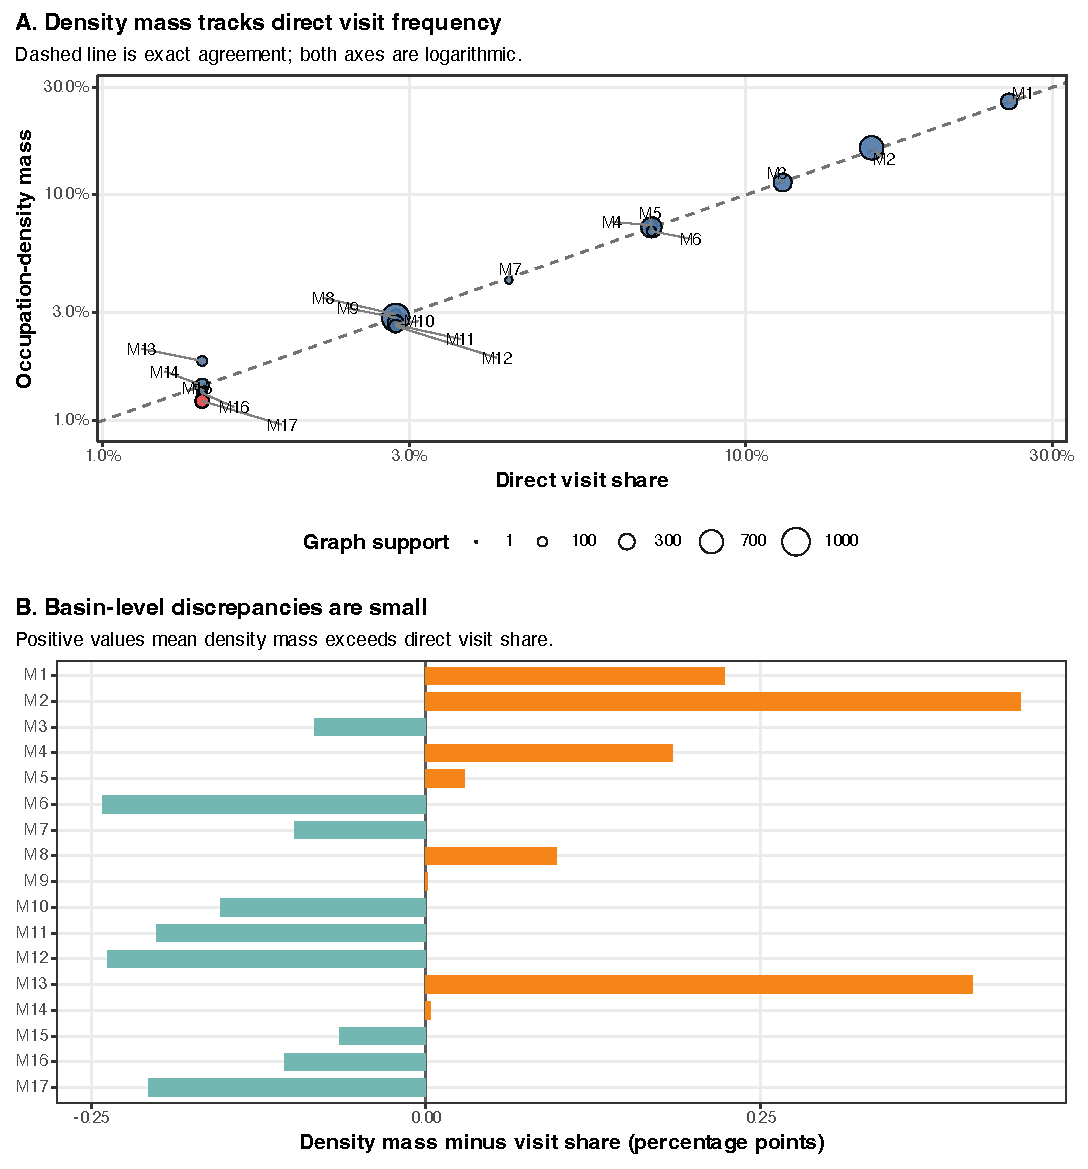
\includegraphics[width=\linewidth]{figures/density_mass_vs_direct_visits.pdf}
  \caption{Comparison of reconstructed occupation-density mass with direct
  Subject 15 visit frequency.  M17 is highlighted in red.  The density estimate
  and raw visit distribution agree closely, despite being conceptually
  distinct summaries.}
  \label{fig:mass-visits}
\end{figure}

\subsection{The 17 directly observed basins}

\begin{longtable}{
  @{}l
  S[table-format=4.0]
  S[table-format=4.0]
  S[table-format=2.0]
  S[table-format=1.0]
  S[table-format=1.0]
  S[table-format=2.2]
  S[table-format=2.1]@{}
}
\caption{Characteristics of all maximum basins with at least one direct
Subject 15 visit.  ``Mass'' is percentage occupation-density mass; ``Days'' is
midpoint exposure and is descriptive only.}
\label{tab:top17}\\
\toprule
{Basin} & {Peak vertex} & {Graph support} & {Visits} &
{Runs} & {Longest run} & {Mass (\%)} & {Days} \\
\midrule
\endfirsthead
\multicolumn{8}{l}{\small\itshape Table \thetable{} continued}\\
\toprule
{Basin} & {Peak vertex} & {Graph support} & {Visits} &
{Runs} & {Longest run} & {Mass (\%)} & {Days} \\
\midrule
\endhead
\midrule
\multicolumn{8}{r}{\small\itshape Continued on next page}\\
\endfoot
\bottomrule
\endlastfoot
M1 & 1598 & 316 & 18 & 8 & 5 & 25.94 & 18.0 \\
M2 & 1628 & 715 & 11 & 5 & 7 & 16.16 & 11.0 \\
M3 & 1635 & 399 & 8 & 2 & 7 & 11.35 & 8.5 \\
M4 & 1575 & 141 & 5 & 4 & 2 & 7.33 & 5.5 \\
M5 & 1641 & 517 & 5 & 3 & 3 & 7.17 & 5.0 \\
M6 & 1578 & 95 & 5 & 3 & 3 & 6.90 & 5.0 \\
M7 & 1609 & 55 & 3 & 3 & 1 & 4.19 & 3.0 \\
M8 & 1603 & 118 & 2 & 2 & 1 & 2.95 & 2.0 \\
M9 & 1622 & 1003 & 2 & 2 & 1 & 2.86 & 2.5 \\
M10 & 1590 & 312 & 2 & 1 & 2 & 2.70 & 2.0 \\
M11 & 1614 & 32 & 2 & 1 & 2 & 2.66 & 2.0 \\
M12 & 1621 & 197 & 2 & 1 & 2 & 2.62 & 2.0 \\
M13 & 1638 & 107 & 1 & 1 & 1 & 1.84 & 1.0 \\
M14 & 1574 & 217 & 1 & 1 & 1 & 1.43 & 0.5 \\
M15 & 1618 & 98 & 1 & 1 & 1 & 1.36 & 1.0 \\
M16 & 1640 & 126 & 1 & 1 & 1 & 1.32 & 1.0 \\
M17 & 1589 & 1 & 1 & 1 & 1 & 1.22 & 1.0 \\

\end{longtable}

M1 is both the most massive and most frequently visited basin.  The table also
shows why no single support quantity is sufficient: M9 contains \num{1003}
graph vertices but only two direct visits, whereas M17 contains one graph
vertex and one direct visit.

\subsection{Graph support is not empirical trajectory support}

Across M1--M17, graph support and direct visit count have Spearman correlation
$\rho=\SupportVisitSpearman$, much weaker than the mass--visit association.
Graph support measures the size of a geometric attraction set over every
vertex in the smoothed ambient graph.  Direct visit count measures how many
observed subject states land in that set.  The two may diverge because the
graph contains interpolating or other-subject states, sampling is sparse, and
\textsc{closest} routing is determined by local edge lengths.

\begin{figure}[htbp]
  \centering
  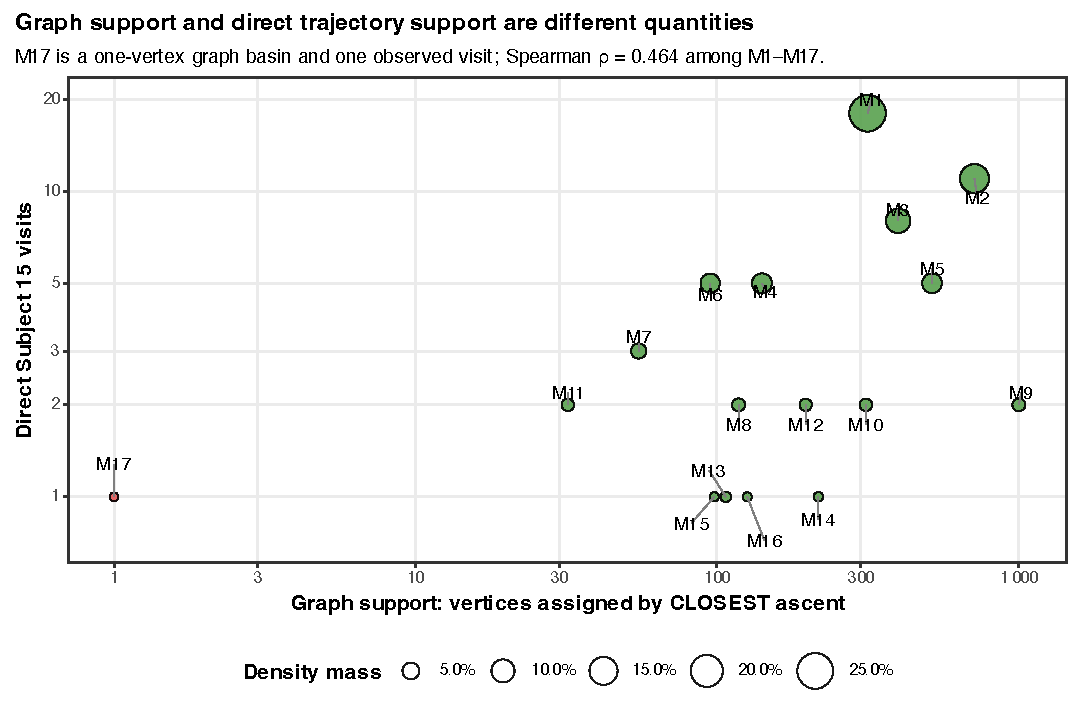
\includegraphics[width=0.82\linewidth]{figures/graph_support_vs_direct_visits.pdf}
  \caption{Graph support versus direct Subject 15 visit count for M1--M17.
  Point area represents density mass.  M17 is highlighted in red.}
  \label{fig:support-visits}
\end{figure}
\FloatBarrier

\subsection{Why M17 can have support one}

M17 is the strict local maximum at vertex 1589.  Its peak and density mass are
both \num{0.0122134}; it is mass rank 17, graph-support rank 304, and has
prominence \num{0.00196728}.  It merges into M1 at field level
\num{0.0102461}.  The only direct Subject 15 visit is time index 16
(\texttt{UAB015\_W3D2}, state S3, CST IV-B), representing one midpoint day.

The apparent paradox disappears when the local routing definition is applied.
All three neighbors lie below M17, so vertex 1589 is a local maximum and roots
at itself.  Yet each neighbor has a different higher vertex connected by a
shorter edge than its edge to M17.  Consequently, none chooses M17 as its
\textsc{closest} ascending successor.

\begin{table}[H]
\centering
\caption{Exact local \textsc{closest} routing around M17 (vertex 1589).
``Chosen length'' is the edge to the selected higher successor; ``M17 length''
is the edge from that source vertex to M17.}
\label{tab:m17-neighbors}
\begin{tabular}{
  @{}S[table-format=4.0]
  S[table-format=1.6]
  S[table-format=4.0]
  S[table-format=1.5]
  S[table-format=1.5]
  l@{}
}
\toprule
{Source} & {Field} & {Chosen successor} & {Chosen length} &
{M17 length} & {Final root} \\
\midrule
1588 & 0.008493 & 1584 & 0.07211 & 0.10430 & M1 \\
1592 & 0.010246 & 1597 & 0.08153 & 0.08246 & M1 \\
1593 & 0.010246 & 1592 & 0.05646 & 0.11791 & M1 \\
\bottomrule
\end{tabular}

\end{table}

Thus support one is not an error: $B_{\mathrm{M17}}=\{1589\}$.  It is evidence
that smooth catchment intuition does not transfer automatically to a
nonsmooth finite graph.  M17 remains empirically relevant because the subject
actually visits its root once; many numerical-tail singleton basins do not.

\subsection{Visit-threshold sensitivity}

A direct-support threshold is scientifically interpretable but it changes the
estimand.  The following is a sensitivity analysis, not a recommended final
cutoff.

\begin{table}[htbp]
\centering
\caption{Consequences of requiring a minimum number of direct Subject 15
visits.  Coverage columns are percentages.}
\label{tab:thresholds}
\begin{tabular}{
  @{}S[table-format=2.0]
  S[table-format=2.0]
  S[table-format=2.0]
  S[table-format=3.1]
  S[table-format=2.1]
  S[table-format=3.1]
  S[table-format=3.1]@{}
}
\toprule
{Min. visits} & {Basins} & {Visits} & {Visit coverage} &
{Days} & {Time coverage} & {Mass coverage} \\
\midrule
1 & 17 & 70 & 100.0 & 71.0 & 100.0 & 100.0 \\
2 & 12 & 65 & 92.9 & 66.5 & 93.7 & 92.8 \\
3 & 7 & 55 & 78.6 & 56.0 & 78.9 & 79.0 \\
5 & 6 & 52 & 74.3 & 53.0 & 74.6 & 74.8 \\
10 & 2 & 29 & 41.4 & 29.0 & 40.8 & 42.1 \\
\bottomrule
\end{tabular}

\end{table}

\begin{figure}[htbp]
  \centering
  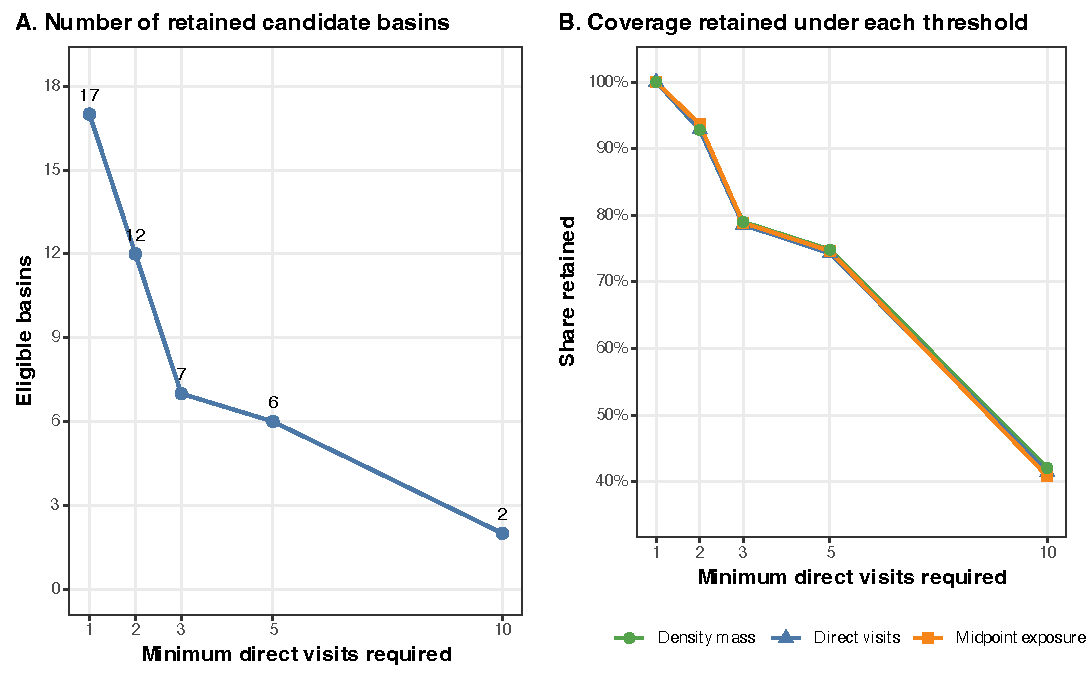
\includegraphics[width=\linewidth]{figures/visit_threshold_sensitivity.pdf}
  \caption{Sensitivity of the candidate EOT set and retained coverage to a
  direct-visit threshold.  Visit, midpoint-exposure, and density-mass coverage
  remain similar for this subject.}
  \label{fig:thresholds}
\end{figure}

Requiring at least two visits retains 12 basins and about 93\% of visits,
midpoint exposure, and density mass.  Requiring at least three retains seven
basins and about 79\% of each.  A hard threshold therefore provides
interpretability at the cost of discarding genuine low-frequency states such
as M17.  A more defensible final rule may use a primary visit threshold plus an
explicit rare-state category or stability criterion.

\subsection{Temporal organization}

Counts alone do not distinguish one sustained episode from repeated returns.
The observed sequence shows both long occupancy blocks and isolated visits.
M17 is a single observed state, while M1 occurs in eight runs and M2 in five.
This motivates reporting run count and persistence alongside total visits.

\begin{figure}[htbp]
  \centering
  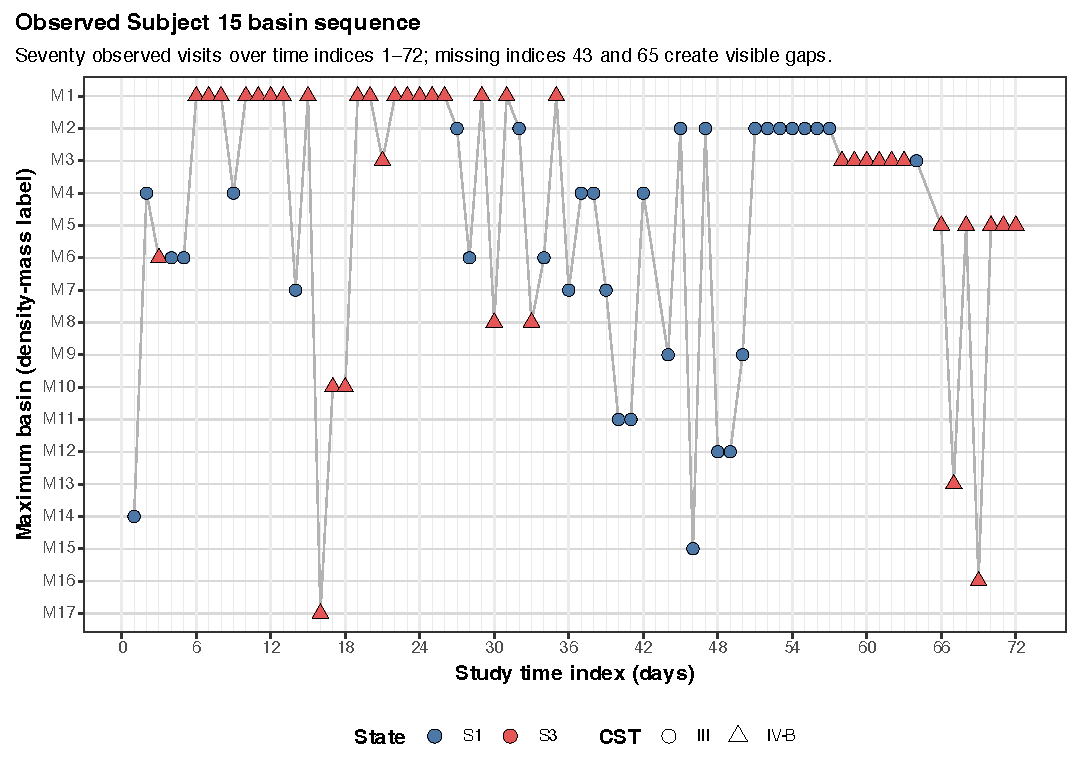
\includegraphics[width=\linewidth]{figures/observed_basin_sequence.pdf}
  \caption{Temporal sequence of directly observed basin assignments.
  Horizontal position is study time index; vertical position is the
  density-mass basin label.  Color and shape retain the observed state and CST
  annotations.}
  \label{fig:sequence}
\end{figure}
\FloatBarrier

\section{Implications for elementary occupation types}

The evidence supports a two-stage interpretation:
\begin{enumerate}
  \item \textbf{Candidate construction.}  Use the canonical \textsc{closest}
  reconstruction to partition the occupation-density field into geometrically
  well-defined attraction basins.
  \item \textbf{Scientific qualification.}  Decide which candidates count as
  major EOTs using subject-facing evidence: direct visit count or share,
  temporal persistence and returns, density mass, and stability across
  smoothing or graph scales.
\end{enumerate}

This separation preserves the mathematical value of the canonical basin
complex without asserting that every discrete local maximum is an elementary
occupation type.  It also makes the choice of estimand explicit:
\begin{itemize}
  \item \textbf{Visit-weighted EOT prevalence} treats each observed state
        equally and answers how frequently sampled states fall in each basin.
  \item \textbf{Duration-weighted occupation} uses represented time and moves
        toward a time-occupation or quasi-equilibrium target.  It is useful as
        sensitivity analysis but should not silently replace an EOT frequency
        estimand.
  \item \textbf{Graph support} describes the ambient reconstructed field and
        should not be interpreted as subject trajectory support.
\end{itemize}

For this data set, raw visit share and midpoint-weighted share are close, so
the practical ranking is robust to the simple duration weighting.  That
agreement is an empirical result for Subject 15, not a general equivalence.

\section{Recommended next analysis}

Before fixing a universal EOT rule, the next comparison should be repeated
across subjects and smoothing scales.  For each candidate basin, record:
\begin{enumerate}
  \item direct visits, visit share, runs, longest run, and returns;
  \item midpoint or interval exposure as a separate duration-sensitive
        summary;
  \item density mass, peak value, prominence, and graph support;
  \item survival and label stability across graph and field scales.
\end{enumerate}
Candidate decision rules can then be compared by retained density mass,
retained direct visits, temporal reproducibility, and cross-scale stability.
The threshold table in this report is deliberately illustrative; it does not
select a final biological cutoff.

\section{Limitations}

This is a single-subject case study.  The graph and occupation-density field
depend on upstream embedding, graph construction, connectivity repair,
smoothing, and normalization choices.  Midpoint weights interpolate
represented time but do not model unobserved transitions.  Direct visit counts
are also sample-design dependent.  Finally, no external biological validation
is used here; the conclusions concern the relationship among reconstruction
geometry, density mass, and observed trajectory support.

\section{Reproducible artifacts}

The report is rebuilt by
\path{dev/subject15_eot_comparison_2026-08-06/latex_report/build_subject15_eot_comparison_report.sh}.
Its figure builder consumes only regenerated CSV/RDS analysis outputs.  The
principal machine-readable artifacts are:
\begin{itemize}
  \item \path{subject15_maximum_basin_eot_comparison.csv}: all 352 maximum
        basins and all reported characteristics;
  \item \path{subject15_visit_basin_assignments.csv}: all 70 observed visits;
  \item \path{subject15_eot_visit_threshold_sensitivity.csv}: threshold
        sensitivity;
  \item \path{subject15_m17_local_flow.csv}: exact local M17 routing evidence.
\end{itemize}
All artifact paths are relative to
\path{dev/subject15_eot_comparison_2026-08-06/}.

\end{document}
